% -*- TeX-master: "../all_the_notes.tex" -*-

\section{Linbalnd operators covered in depth\label{sec:linbland2}}
This section  will cover how  we derive these  $ L_j $  operators which
were used in Sec.~\ref{subsec:dynamics_with_pauli}.
\subsection{Pure dephasing\label{sec:lin_1}}
Let us consider  a two level system, whose Hamiltonian  is undergoing a
fluctuation in time due to \red{movement of the energy levels}
\begin{equation}\label{eq:lin_2}
  \mathcal{H} = \imatrixTwoColTwoRow{\red{\epsilon(t)}}{0}{0}{0} \iratext{eigenstates}
  \begin{aligned}
    \iket{0}     &     =     \imatrixTwoCol{0}{1}\\\iket{1}     &     =
    \imatrixTwoCol{1}{0}
  \end{aligned}
\end{equation}

\noindent  Under  free  evolution  an  arbitrary  state  \iket{\Psi(0)}  =
a\iket{1} + b\iket{0} will evolve to:

\begin{equation}\label{eq:lin_3}
  \begin{aligned}
    \iket{\Psi(t)} & = \prod_i U(\Delta t_i) \iket{\Psi(0)} \\
    & = \prod_i \exp\left[-i\frac{\epsilon(\Delta t_i)}{\hbar} \imatrixTwoColTwoRow{1}{0}{0}{0}\right]\imatrixTwoCol{a}{b}\\
    & = \prod_i \bigg(\mathbb{I}\imatrixTwoCol{a}{b} + \blue{\sum_{{N = 1}}\frac{\left[\frac{-i\epsilon(\Delta t_i)}{\hbar}\right]^N}{N!} \imatrixTwoColTwoRow{1}{0}{0}{0}\imatrixTwoCol{a}{b}}\bigg)\\
    & = \prod_i \bigg(\imatrixTwoCol{a}{b} + \blue{\exp\left[-i\frac{\epsilon(\Delta t_i)}{\hbar}\right]\imatrixTwoCol{a}{0} - \imatrixTwoCol{a}{0}\bigg)}\\
    & = \prod_i \imatrixTwoCol{e^{-i\frac{\epsilon(\Delta t_i)}{\hbar}}a}{b} = \imatrixTwoCol{e^{-i\sum_i\frac{\epsilon(\Delta t_i)}{\hbar}}a}{b} \\
    &     \red{=     \imatrixTwoCol{ae^{i\varphi}}{b}     \qquad     \varphi     =
      -\int_{0}^{t}\frac{\epsilon(t')}{\hbar}dt'}
  \end{aligned}
\end{equation}

\begin{framed}\noindent
  \noindent Thus, free  evolution under a fluctuating  energy will lead
  to a phase accumulation between the two states:
  \begin{equation}\label{eq:lin_4}
    \ket{\Psi} = a\red{e^{i\varphi}}\iket{1} + b\iket{0} =  \imatrixTwoCol{a\red{e^{i\varphi}}}{b}
  \end{equation}

  \noindent which we can probe by measuring the \isigmax\ component and
  see this integrated phase:

    \begin{equation}\label{eqn:lin_1}
      \isigmax = ab^{*}\red{e^{i\varphi}} + a^{*}b\red{e^{-i\varphi}} \iratext{a,b real} 2ab\cos(\varphi).
    \end{equation}

  \end{framed}

  \newpage
  \paragraph{Single  run}  Each  measurement  of  $  \sigma_x  $  gives
  $  \pm1   $  with  probabilities  (projecting   onto  the  respective
  eigensubspaces):

  \begin{equation}
    \begin{aligned}
      &P(1) = \iabsSquared{\bra{\Psi}\left(\frac{\iket{0} + \iket{1}}{\sqrt{2}}\right)} = \frac{1}{{2}}\iabsSquared{ae^{-i\varphi} + b} = \frac{1}{2}\left({a}^2 + {b}^2 + 2ab\cos(\varphi) \right)\\
      & P(-1) = \frac{1}{2}\left(a^2 + b^2 - 2ab\cos(\varphi)\right)
    \end{aligned}
  \end{equation}

              \begin{figure}[ht]
                \centering 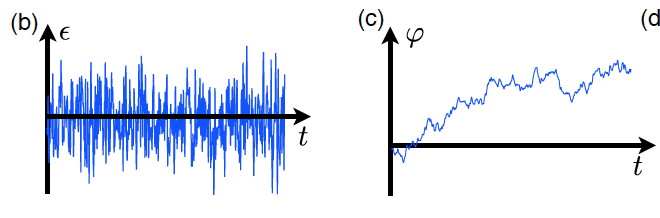
\includegraphics[height=3cm]{lin_1}
                \caption{The energy of the two levels fluctuates around
                  0.   Integration  will  give a  unique  phase  value,
                  $ \phi =  -\int_0^t\frac{\epsilon(t')}{\hbar}dt' $, that determines
                  collapse  probability. \textbf{This  is for  a single
                    run.}}
              \end{figure}

              \paragraph{Averaging} Averaging  over the $ \pm  1 $ will
              allow      us      to      recover      the      \isigmax
              $ \propto \cos(\varphi) $ dependence.
              \begin{itemize}
              \item Each run  has an independent $ \epsilon(t) $  and hence an
                independent $ e^{i\varphi} $;
              \item Averaging will thus result in the classical average
                \iaverage{e^{i\varphi}}$ _\varphi $.
              \end{itemize}

              \begin{framed}\noindent
                \noindent  And   thus  Eq.~\eqref{eqn:lin_1}   will  in
                practise be reading:

  \begin{equation}\label{eq:linrelax_10}
    \isigmax = ab^{*}\blue{\iaverage{e^{i\varphi}}_\varphi} + a^{*}b\iaverage{e^{-i\varphi}}_\varphi \iratext{a,b real} 2ab\cos(\iaverage{\varphi}_\varphi).
  \end{equation}
\end{framed}

\noindent Let us label this interference term factor

  \begin{equation}\label{eq:linrelax_11}
    v(t) = \blue{\iaverage{e^{i\varphi}}_\varphi},
  \end{equation}

  \noindent   which  is   reflective   of  the   noise  supression   of
  interference: $ \blue{v(t)} \rightarrow 0 $.

  \begin{figure}[ht]
    \centering 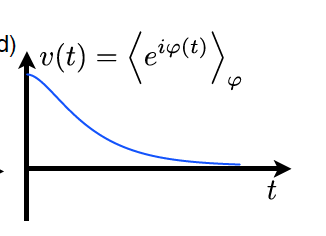
\includegraphics[height=3cm]{lin_2}
    \caption{The  longer we  allow  the phase,  $ \varphi  $,  to evolve  the
      greater amount  of cancellation  between the independent  runs we
      shall get.  In  this way and interference that we  can infer will
      wash out.\label{fig:lin_2}}
  \end{figure}

  \noindent \red{\paragraph{Why  does it  decrease with  time?}  Making
    the assumption that $ \epsilon(t) $ fluctuates around 0 we will find
    that %$ \varphi $ can be expanded:

    % \begin{equation}\label{key}
    %             \iaverage{\varphi(t)}_\varphi           =
    %             \iaverage{\varphi(0)}_\varphi           +
    %                 %             t\iaverage{\frac{d\varphi}{dt}|_{t=0}}_\varphi
    %                 %             +
    %                 %             \frac{t^2}{2}\iaverage{\frac{d^2\varphi}{dt^2}|_{t=0}}_\varphi
    %                 %             + \cdots
    % \end{equation}
%
    % \noindent and because
    \begin{itemize}
    \item                         Initially                         any
      $ \varphi(0)  = -\int_{0}^{0}\frac{{\epsilon(t')}}{\hbar}dt' =  0 $ (no  phase has
      been allowed to accumulate) and therefore
      \begin{equation}\label{key}
        \iaverage{e^{i\varphi(0)}}_\varphi = 1.
      \end{equation}
    \item Subsequently, the random evolution of the phase will lead to

      \begin{equation}\label{key}
        \begin{aligned}
          \iaverage{e^{i\varphi(t)}}_\varphi & = e^{i\phi_1(t)} + e^{i\phi_2(t)} + e^{i\phi_3(t)} + \cdots\\
          & = x_1 + iy_1 + x_2 + iy_2 + x_3 + iy_3 + \cdots\\
          & = \iaverage{x} + i\iaverage{y}\\
          & = 0 + i0 = 0
        \end{aligned}
      \end{equation}

      \noindent and  thus perfect cancellation -  any agreement between
      the states will persists only for short times.
    \end{itemize}}

 \subsection{Pure dephasing from partial trace\label{sec:lin_2}}
 We  can  arrive  at  Eq.~\eqref{eqn:lin_1} in  a  similar  fashion  by
 considering a system-bath state

   \begin{equation}\label{key}
     \ket{\Psi_{SB}} = \ket{\Psi} \otimes \ket{\chi_B} \quad\text{where}\quad
     \begin{aligned}
       \Ket{\Psi} & = a\iket{1} + b\iket{0}\\
       \ket{\chi} & = \sum_i\sqrt{w_i}\ket{\chi_j}
     \end{aligned}
   \end{equation}

   \noindent   where  the   bath   is  a   weighted  superposition   of
   \iket{\chi_i} states (normalised of course).

   \begin{framed}\noindent
     \noindent We postulate,  that the state of the  system will evolve
     acoording to the state of the bath:
     \begin{equation}\label{key}
       \begin{aligned}
         U_{SB}(t)\iket{1}\ket{\chi_i} & = \red{e^{i\varphi_i(t)}}\iket{1}\ket{\chi_i}\\
         U_{SB}(t)\iket{0}\ket{\chi_i} &=\iket{0}\ket{\chi_i}\\
       \end{aligned}
     \end{equation}
     \noindent  acquiring  a phase  only  for  the \iket{1}  state  and
     depending on the states of the bath.
   \end{framed}

   \noindent Thus we shall get the following evolution:
   \begin{equation}\label{key}
     \begin{aligned}
       \ket{\Psi_{SB}(t)} & = aU_{SB}(t)\left[\sum_i\sqrt{w_i}\ket{1}\ket{\chi_i}\right] + bU_{SB}(t)\left[\sum_i\sqrt{w_i}\ket{0}\ket{\chi_i}\right]\\
       & = a\iket{1}\red{\sum_i\sqrt{w_i}e^{i\varphi_i(t)}\ket{\chi_i}} + b\iket{0}\blue{\sum_i\sqrt{w_i}\ket{\chi_i}}\\
       & = a\iket{1}\red{\ket{\chi_1}} + b\iket{0}\blue{\ket{\chi_0}}
     \end{aligned}
   \end{equation}
   \vspace{1cm}

   \noindent   Taking   the   experctation  value   of   the   operator
   $ \mathbb{I} \otimes  \sigma_x $, where we only operate  on the system, we
   get

   \begin{equation}\label{key}
     \begin{aligned}
       \iaverage{\sigma_x}_S & = \bra{\Psi_{SB}(t)}\mathbb{I} \otimes \sigma_x\ket{\Psi_{SB}(t)} \\
       & = ab^{*}\blue{\bra{\chi_0}}\red{\ket{\chi_1}} + a^{*}b\red{\bra{\chi_1}}\blue{\ket{\chi_0}}\\
       & = \sum_iw_iab^{*}e^{i\varphi_i(t)} + cc.\\
       & = \red{ab^{*}\iaverage{e^{i\varphi(t)}}_\varphi + cc.}
     \end{aligned}
   \end{equation}

   \noindent                                                      where
   \red{$ \iaverage{e^{i\varphi(t)}}_\varphi  = \sum_iw_ie^{i\varphi_i}
     =  \blue{\bra{\chi_0}}\red{\ket{\chi_1}}$}  and   we  recover  the
   result Eq.~\eqref{eqn:lin_1}.  See how  the environment picks up the
   state of the system

 \subsection{General roundup}
 In  Sec.~\ref{sec:lin_1}  and  \ref{sec:lin_2}  we have  come  to  two
 equivalent ways of recovring the state of the system:

  \begin{equation}\label{key}
    \ket{\Psi(t)}_\varphi = a\iket{1}\red{v(t)} + b\iket{0}.
  \end{equation}

  \noindent       where      the       phase      supression       term
  $ \red{v(t) = \iaverage{e^{i\varphi}}_\varphi} $ is a consqeuence of:

  \begin{itemize}
  \item Classical noise process as  we average over different runs that
    acquire different phases
    \begin{equation}\label{key}
      \ket{\Psi(t)}_\varphi = \red{\sum_i} a\iket{1}\red{e^{i\varphi_i(t)}} + b\iket{0}.
    \end{equation}
  \item Quantum mechanical Interaction  with the weighted superposition
    of the bath states \iket{\chi_i},
    \begin{equation}\label{key}
      \begin{aligned}
        \ket{\Psi}_\phi & =  a\iket{1}{\sum_i\sqrt{w_i}e^{i\varphi_i(t)}\ket{\chi_i}} + b\iket{0}{\sum_i\sqrt{w_i}\ket{\chi_i}}\\
        &     =      \left[a\iket{1}\red{\sum_ie^{i\varphi_i(t)}}     +
          b\iket{0}\right]\ket{\chi}
      \end{aligned}
    \end{equation}
  \end{itemize}

  \begin{framed}\noindent
    \noindent Let us represent the state as a density matrix

  \begin{equation}\label{key}
    \rho(t) = \imatrixTwoColTwoRow{\iabsSquared{a}}{ab^{*}\red{v(t)}}{a^{*}b\red{v^{*}(t)}}{\iabsSquared{b}},
  \end{equation}

  Where   we  see   that  dephasing   affects  only   the  off-diagonal
  elements. Taking the purity

  \begin{equation}\label{key}
    \begin{aligned}
      \itrace{\rho^2} & = \iabs{a}^4 + 2\iabsSquared{a}\iabsSquared{b}\iabsSquared{v(t)} + \iabs{b}^4\\
      & = (\iabsSquared{a}+\iabsSquared{b})^2 - 2\iabsSquared{a}\iabsSquared{b} + 2\iabsSquared{a}\iabsSquared{b}\iabsSquared{v(t)}\\
      &                    =                     1                    -
      2\iabsSquared{a}\iabsSquared{b}\left(1-\iabsSquared{v(t)}\right),
    \end{aligned}
  \end{equation}

  \noindent   and    as   $    v(t)   \rightarrow   0    $   the    purity   goes
  $ 1 \rightarrow 1/2 $ if we start from an even superposition.
\end{framed}

\noindent Let  us assume  that the  phase suppresion  term falls  as an
exponential (which we kind of show in Fig.~\ref{fig:lin_2})

  \begin{equation}\label{key}
    v(t) = \iaverage{e^{i\varphi(t)}}_\varphi = e^{-\Gamma_{\varphi}t}
  \end{equation}

  \noindent in which case we can write

  \begin{equation}\label{eqn:lin_3}
    \dot{\rho}_{10}(t) = -\Gamma_{\varphi}\rho_{10}(t).
  \end{equation}

  \noindent \textbf{We want  to incorporate this into  the evolution of
    the form}
  \begin{equation}\label{eq:linrelax_5}
    \mathbf{\mathcal{L}[\rho(0)] = \rho(t)}.
  \end{equation}
  \subsection{Relaxation in the Linbland Equation}
  However, the Linbalnd  equation, incorporating Eq.~\eqref{eqn:lin_3},
  cannot  be  written arbitraraly,  because  the  density matrix  is  a
  weighted \textbf{probability} superposition

  \begin{equation}\label{eq:linrelax_1}
    \rho = \sum_i\iketbra{\psi_i}{\psi_i},
  \end{equation}

  \noindent and therefore cannot have negative eigenvalues.  If we, for
  example,  take  the  decay  of  a state  with  initial  off  diagonal
  elements:

  \begin{equation}\label{eq:linrelax_2}
    \imatrixTwoColTwoRow{\rho_{00}(0)}{\rho_{01}(0)}{\rho_{10}(0)}{\rho_{11}(0)} \ira \imatrixTwoColTwoRow{0}{\rho_{01}(t)}{\rho_{10}(t)}{1} \red{\rightarrow \text{negative eigenvalues!}}
  \end{equation}

\begin{framed}\noindent
  An arbitrary operator $ \Phi $ has to be a completely positive:
  \begin{equation}\label{eq:linrelax_3}
    \begin{aligned}
      \Phi(\rho) & \ge 0\\
      \Phi : & B(\mathcal{\tilde{H}}) \ira B()\mathcal{\tilde{H}})\\
      & \text{where } \mathcal{\tilde{H}} = \mathcal{{H}} \otimes \mathcal{H'}\\
      & \text{and }  \Phi \text{ acts on one product  space and leaves the
        other untouched}
    \end{aligned}
  \end{equation}

\end{framed}

\noindent This is fullfilled by the Kraus operator:

  \begin{equation}\label{eq:linrelax_4}
    \Phi(\rho) = \sum_iK_i\rho K_i\idagger\qquad \sum_iK_i\idagger K_i = \mathbb{I}.
  \end{equation}

  \noindent A great  example is unitary evolution $ K  = U(t) $, random
  unitary evolution  $ K_i = \sqrt{w_i}U_i(t)  $ or the evolution  of a
  system batch state:

  \begin{equation}
    \begin{aligned}
      \rho(t) & = \itrace{U_{SB} \rho_S\otimes\iketbra{\chi_B(0)}{\chi_B(0)}U_{SB}\idagger}\\
      & = \sum_j\left[\bra{\chi_j}U_{SB}\iket{\chi_B(0)}\right]\rho_{S}\bra{\chi_{B}(0)U_{SB\idagger}\iket{\chi_j}}\\
      & = \sum_j K_j\rho_{S}K_j\idagger,
    \end{aligned}
  \end{equation}

  \noindent where the Kraus operators describe the traced out effect of
  the Bath state evolution.  The full Hamiltonian reads:

 \begin{equation}\label{eq:linrelax_6}
   \dot{\rho}(t) = -\frac{i}{\hbar}\icommutation{\mathcal{H}}{\rho} + \sum_j\left(R_j\rho R_j\idagger - \frac{1}{2}\rho R_j\idagger R_j - \frac{1}{2}\rho R_j\idagger R_j\right)
 \end{equation}


\begin{framed}\noindent
  Usually, relaxation  operators are of  a simple form,  describing the
  operator that  induces the dissipative transition,  multiplied by the
  square root of the corresponding  rate.  \red{The decay rates must be
    much smaller than the transition frequencies of the system.}
  \begin{itemize}
  \item  \textbf{Pure  dephasing}  due  to  energy  level  fluctuations
    \red{as we set out to  show in Eq.~\eqref{eqn:lin_3}} is associated
    with the $ \sigma_z $ term
    \begin{equation}\label{eq:linrelax_7}
      R = \sqrt{\frac{\Gamma_{\varphi}}{2}}\sigma_z.
    \end{equation}

    \noindent which leads to relaxation terms

    \begin{equation}\label{eq:linrelax_8}
      \begin{aligned}
        &R\rho R\idagger - \frac{1}{2}R\idagger R - \frac{1}{2}\rho R\idagger R\\
        &                                                             =
        \Gamma_{\varphi}\imatrixTwoColTwoRow{0}{-\rho_{01}}{-\rho_{10}}{0}.
      \end{aligned}
    \end{equation}

    \noindent It recovers the decaying  off diagonal dynamics, and that
    is good enough for me.

  \item \textbf{Exponential  relaxation} from excited to  ground state,
    is ossicated with $ \sigma_{-} = \iketbra{0}{1}$

    \begin{equation}\label{key}
      R = \sqrt{\Gamma}\sigma_{-}
    \end{equation}

    \noindent giving

    \begin{equation}\label{eqn:lin_5}
      \Gamma\imatrixTwoColTwoRow{+\rho_{11}}{\red{-\frac{1}{2}\rho_{01}}}{\red{-\frac{1}{2}\rho_{10}}}{-\rho_{11}},
    \end{equation}

    \noindent   which  results   in   non-trivial  \red{off   dioagonal
      elements}, which is exactly 1/2 of the decay rate.
  \end{itemize}

  Combining the effect of  diagonal terms in Eq.~\eqref{eq:linrelax_8},
  \eqref{eqn:lin_5} we define

  \begin{equation}\label{key}
    \Gamma_2 = \Gamma_{\varphi} + \frac{\Gamma_1}{2}
  \end{equation}
\end{framed}
\newpage

%%% Local Variables:
%%% mode: latex
%%% TeX-master: "../all_the_notes"
%%% End:
